\documentclass[../../main.tex]{subfiles}

\begin{document}

ETC o Extracción, Transformación y Carga (ETC) es un proceso de integración de datos desde múltiples fuentes con la finalidad de construir un almacén de datos.

\begin{figure}[h]
\centering
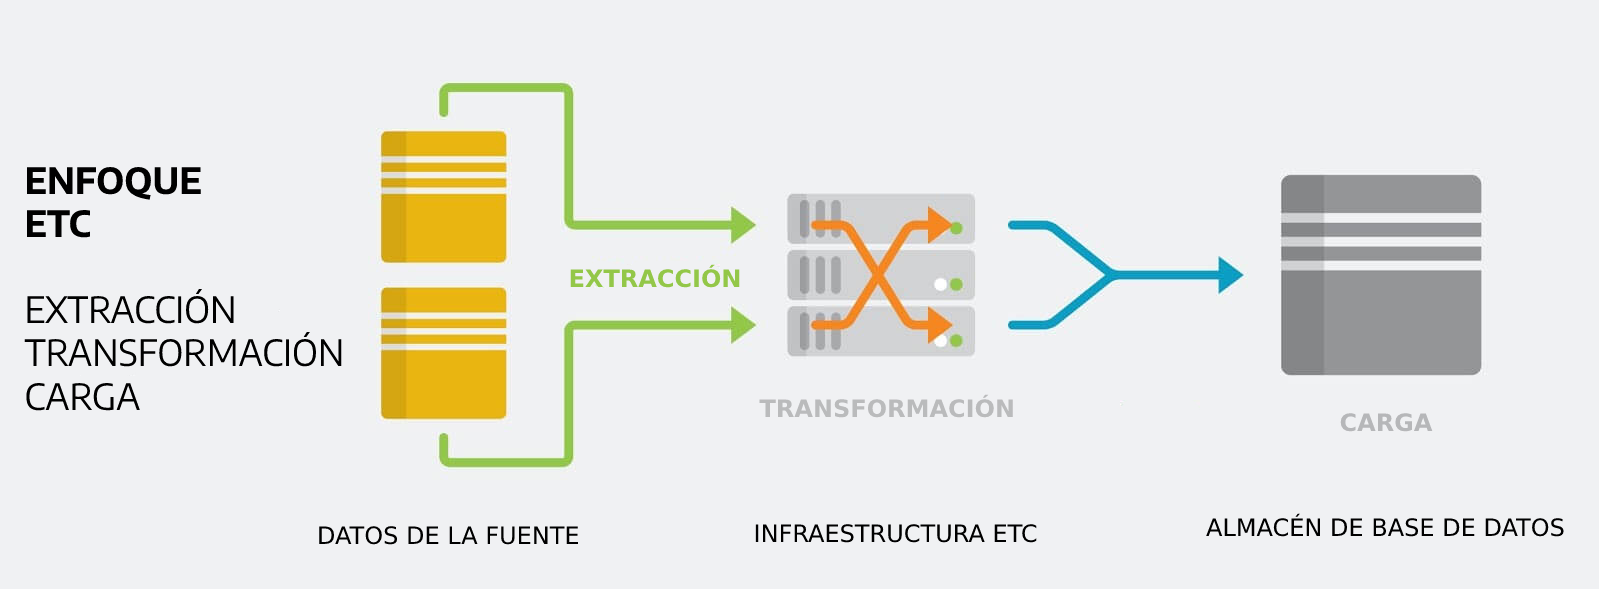
\includegraphics[width=1\textwidth]{images/4_sistema/etl.png}
\caption{Proceso ETC}
\end{figure}

Este proceso se divide en tres fases diferentes:

\begin{itemize}
    \item \textbf{Extracción}: Esta fase se encarga de obtener los datos deseados desde los múltiples fuentes.
    \item \textbf{Transformación}: Fase en el cual se transforma los datos obtenidos para mantener una consistencia entre los datos y que sea más fácil de manejar.
    \item \textbf{Carga}: Fase en la que se carga los datos transformados en un servidor o almacén de base de datos.
\end{itemize}


En este caso para el proyecto la extracción de los datos se hará realizando peticiones HTTP de tipo GET a la API de las redes sociales.ºº

\subsubsection{Reddit}

Reddit\cite{doc18} es una plataforma en la cual se combina contenidos web, noticias sociales, foros y una red social con una gran multitud de usuarios de diferentes partes del mundo.

La forma en la que se destacan las publicaciones es mediante el sistema de votos, en los cuales cualquier usuario registrado puede dar su voto positivo o negativo a cada publicación , esto permite ver rápidamente aquellas publicaciones que son repudiadas por la comunidad (publicación que tiene una gran cantidad de votos negativos) o que son tendencia en el presente día o las publicaciones con mayor número de votos positivos en un periodo de tiempo (publicaciones que han sido tendencia en el periodo de tiempo especificado).

Esto tiene como resultado que Reddit sea uno de los sitios dónde se publican la gran mayoría de memes y sensaciones virales de todo Internet.\\

A continuación detallamos las peticiones que se utilizan para la obtención de datos de esta red social:

\begin{itemize}

    \item GET \textbf{/user/username/about}
    \begin{itemize}
        \item \textbf{Descripción:} Permite obtener información sobre un usuario que no ha sido eliminado o baneado.
        \item \textbf{Parámetros:}:
        \begin{itemize}
            \item  \textit{username}: dónde se especifica el nombre del usuario a buscar en cuestión.
        \end{itemize}
    \end{itemize}
    
    \item GET \textbf{[/r/subreddit]/comments/article}
    \begin{itemize}
        \item \textbf{Descripción:} Permite obtener los comentarios de un articulo.
        \item \textbf{Parámetros:}:
        \begin{itemize}
            \item  \textit{depth}: especifica la profundidad máxima de los subhilos.
            
            \item  \textit{limit}: limita el número de comentarios a solicitar, el mínimo de elementos que se pueden obtener es 25 y el máximo 100.
            
            \item  \textit{sort}: especifica como se ordena los comentarios, es una opción de la lista (confidence, top, new, controversial, old, random, qa, live).
            
            \item  \textit{sr\_detail}: expande los subreddits.
            
            \item  \textit{article}: código identificador único de cada articulo.
            
            \item  \textit{subreddit}: nombre identificador único del subreddit.
        \end{itemize}
    \end{itemize}
    
    \item GET \textbf{[/r/subreddit]/hot}
    \begin{itemize}
        \item \textbf{Descripción:} Permite obtener las publicaciones que son tendencia a la hora de realizar la petición.
        \item \textbf{Parámetros:}:
        \begin{itemize}
            \item  \textit{limit}: limita el número de publicaciones a solicitar, el mínimo de elementos que se pueden obtener es 25 y el máximo 100.
            
            \item  \textit{show}: con la opción ``all`` muestra todas las publicaciones.
            
            \item  \textit{sr\_detail}: expande los subreddits.
            
            \item  \textit{subreddit}: nombre identificador único del subreddit.
        \end{itemize}
    \end{itemize}
    
    \item GET \textbf{[/r/subreddit]/new}
    \begin{itemize}
        \item \textbf{Descripción:} Permite obtener las publicaciones que son nuevos.
        \item \textbf{Parámetros:}:
        \begin{itemize}
            \item  \textit{limit}: limita el número de publicaciones a solicitar, el mínimo de elementos que se pueden obtener es 25 y el máximo 100.
            
            \item  \textit{show}: con la opción ``all`` muestra todas las publicaciones.
            
            \item  \textit{sr\_detail}: expande los subreddits.
            
            \item  \textit{subreddit}: nombre identificador único del subreddit.
        \end{itemize}
    \end{itemize}
    
    
    \item GET \textbf{[/r/subreddit]/rising}
    \begin{itemize}
    \item \textbf{Descripción:} Permite obtener las publicaciones en los cuales hay mucha actividad reciente con respecto a los comentarios o votos a la hora de realizar la petición.
        \item \textbf{Parámetros:}:
        \begin{itemize}
            \item  \textit{limit}: limita el número de publicaciones a solicitar, el mínimo de elementos que se pueden obtener es 25 y el máximo 100.
            
            \item  \textit{show}: con la opción ``all`` muestra todas las publicaciones.
            
            \item  \textit{sr\_detail}: expande los subreddits.
            
            \item  \textit{subreddit}: nombre identificador único del subreddit.
        \end{itemize}
    \end{itemize}
    
    \item GET \textbf{[/r/subreddit]/top}
    \begin{itemize}
    \item \textbf{Descripción:} Permite obtener las publicaciones en los cuales han tenido los mayores votos durante un periodo de tiempo.
        \item \textbf{Parámetros:}:
        \begin{itemize}
            \item  \textit{t}: limita las publicaciones a un plazo de tiempo determinado, permite como opción lo siguiente: hour, day, week, month, year, all.
            
            \item  \textit{limit}: limita el número de publicaciones a solicitar, el mínimo de elementos que se pueden obtener es 25 y el máximo 100.
            
            \item  \textit{show}: con la opción ``all`` muestra todas las publicaciones.
            
            \item  \textit{sr\_detail}: expande los subreddits.
            
            \item  \textit{subreddit}: nombre identificador único del subreddit.
        \end{itemize}
    \end{itemize}
    
    \item GET \textbf{[/r/subreddit]/sort}
    \begin{itemize}
        \item[$\rightarrow$] \textbf{[/r/subreddit]/top}
        \item[$\rightarrow$] \textbf{[/r/subreddit]/controversial}
    \end{itemize}
    \begin{itemize}
        \item \textbf{Descripción:} Permite obtener ordenar y obtener las publicaciones en un cierto orden.
        \item \textbf{Parámetros:}:
        \begin{itemize}
            \item  \textit{t}: limita las publicaciones a un plazo de tiempo determinado, permite como opción lo siguiente: hour, day, week, month, year, all.
            
            \item  \textit{limit}: limita el número de publicaciones a solicitar, el mínimo de elementos que se pueden obtener es 25 y el máximo 100.
            
            \item  \textit{show}: con la opción ``all`` muestra todas las publicaciones.
            
            \item  \textit{sr\_detail}: expande los subreddits.
            
            \item  \textit{subreddit}: nombre identificador único del subreddit.
        \end{itemize}
    \end{itemize}
    
\end{itemize}

\textit{NOTA: } Remarcar que no es necesario especificar el subreddit en cuestión, es decir, en las peticiones GET si no se quiere delimitar la búsqueda a un subreddit se quita el siguiente texto de la petición ``[/r/subreddit]``. \\

Con la información detallada de cada petición GET ya se puede realizar las peticiones a la API de Reddit para ir obteniendo la información que el usuario solicita.\\
Por ejemplo, se desea realizar la siguiente petición ``\textit{Quiero obtener las 5 publicaciones con mayor votos en el subreddit WorldNews}``, la petición quedaría de la siguiente forma:
\begin{lstlisting}
https://www.reddit.com/r/WorldNews/top?limit=5
\end{lstlisting}

\vskip 0.2in

Para obtener los datos de una forma estructurada en la cual se puede procesar por la aplicación de una forma sencilla posteriormente, es necesario añadir el parámetro ``.json`` a la petición GET que se realice. Esto solicita a la API de Reddit que devuelva el resultado de una petición en un fichero JSON, permitiendo solicitar los datos deseados de forma eficiente, ya que se devuelve el resultado con una estructura y el tiempo de respuesta para obtener dicho fichero es muy pequeño. \\
Por ejemplo, para el caso anterior se quedaría de la siguiente forma:
\begin{lstlisting}
https://www.reddit.com/r/WorldNews/top.json?limit=5
\end{lstlisting}

\vskip 0.2in

Para este proyecto se utiliza el paquete \textit{RedditExtractoR} para obtener los comentarios de una publicación y se utiliza el paquete \textit{jsonlite} para realizar peticiones GET para obtener el resto de la información correspondiente a las publicaciones o usuarios.

De la información obtenida se procesa y se guarda la correspondiente información según el tipo:

\begin{itemize}
    \item \textbf{Publicaciónes:} identificador de la publicación, identificador del subreddit, identificador del autor, título, ratio de votos, total de los premios recibidos, puntuación, fecha creada, fecha añadida, enlace a la publicación, enlace a una web externa si la publicación lo tiene, versión reducida del enlace a la web externa.

    \item \textbf{Comentarios:} identificador de la publicación, identificador del usuario, estructura del comentario, fecha del comentario, puntuación del comentario, texto del comentario.

    \item \textbf{Monedas:} identificador de la moneda, nombre, descripción, precio, recompensa.

    \item \textbf{Premios:} identificador de la publicación, identificador de la moneda, cantidad.
    
    \item \textbf{Usuarios:} identificador del usuario, nombre, fecha creada, fecha añadida, karma total, karma de los comentarios, descripción pública.
\end{itemize}

Algunos procesos que se realizan para mantener una consistencia en los datos pueden ser los siguientes: 
\begin{itemize}
    \item Quitar caracteres no alpha-numericos en los campos de texto.
    \item Cambiar el formato de todas las fechas al formato ISO.
    \item Obtener los identificadores de cada usuario o publicación y modificarlos para su correcta relación.
    \item Comprobar que no se haya insertado una publicación anteriormente, si es el caso no se tratan los datos ni se insertan en el servidor de base de datos.
\end{itemize}

Una vez realizada la petición y se hayan tratado los datos de forma correcta, esta información se inserta en el servidor de base de datos, donde esta sirve para almacenar toda la información correspondiente a cualquier petición que se realice a la API de Reddit, esto con el tiempo se va convirtiendo en una base de datos con un tamaño considerado pero permite obtener mejores resultados a la hora de extraer información, dado que cuanta más datos existan en el servidor de bases de datos, más y mejores relaciones entre los datos se pueden encontrar y obtener.  \\

La base de datos correspondiente a la red social Reddit tiene la siguiente estructura.\\

\begin{figure}[]
\centering
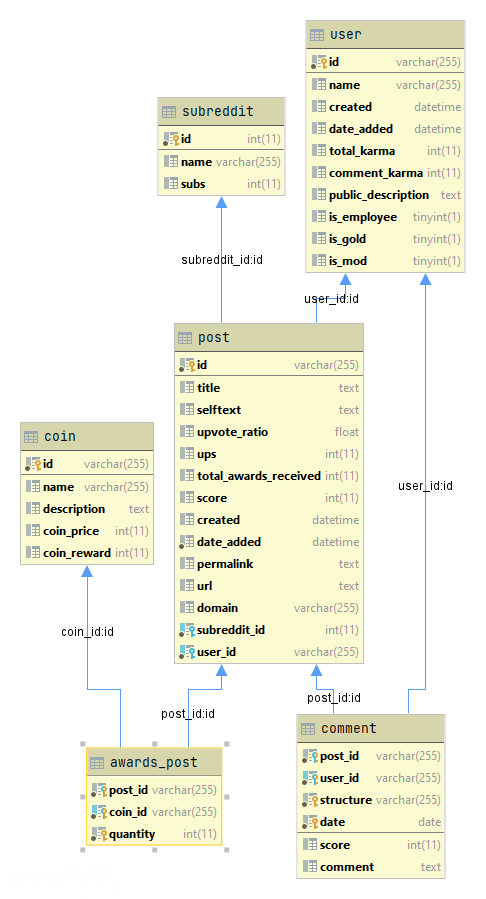
\includegraphics[width=0.7\textwidth]{images/4_sistema/sna_reddit.png}
\caption{Estructura de la base de datos sna\_reddit}
\end{figure}



\end{document}